\chapter{Introduction}
\label{cha:Introduction}


\section{Mathematica as Both a Tool and an Object of Study, at RISC: The Theorema Project}

RISC has a notable relationship to Mathematica: a quick glance at the list of software packages produced by RISC ("Symbolic computation can be seen as the automation and algorithmization of mathematics. Therefore, most of what we do results in concrete software." \cite{noauthor_software_nodate}) demonstrates this: across different branches of Mathematics, many packages are \textit{Mathematica} packages.

The Theorema Project is a long-standing effort originated by Bruno Buchberger and continued by Wolfgang Windsteiger to this day. It will be explored in some detail and with a view to extending it as a collection of Mathematica packages in the following chapter on Theory \ref{cha:Theory}, where this thesis accompanies a practical work, using Wolfram Language (WL) as an engineering tool. Therefore this thesis also has an applications slant, focusing on various aspects of the development of such a package, up to some theory, in rewriting and exploring Theorema particularly.

\subsection{Starting from Rewriting: Mathematica and Wolfram Language as a Programming Language} \label{rewriting}

Mathematica is not Wolfram Language, where in "a first approximation, the Wolfram Language = Mathematica + Wolfram|Alpha [a knowledge-based web service] + Cloud [a storage-oriented web service] + more" \cite{noauthor_wolfram_nodate}, but this disambiguation will be made again in \ref{mm-vs-wl}: at the time Bruno Buchberger was writing, it was the same thing, and it is particularly in "Mathematica as a Rewrite Language" \cite{buchberger_mathematica_1996} that crucial analysis, here from the perspective of the field of rewriting, is made that seems to get to the core of what the language does and can do really well. Under the assumption that it is worth looking at the set of features that make the language stand apart, I would like to follow Buchberger's thoughts on Mathematica as a language for rewriting to begin.

Remarking on the stability of Mathematica, Buchberger observes that "Wolfram's pattern matching is essentially the natural concept of conditional rewriting." \cite[p. 2]{buchberger_mathematica_1996} Writing for an intended audience of both mathematicians in rewriting and Mathematica developers (the groups he poses would benefit from mutual exchange, in \cite{buchberger_mathematica_1996}), Buchberger mostly offeres a definition of the rewriting concept in terms of Mathematica syntax, also useful here. The foundational language constructs according to Buchberger are "constants, ordinary variables, sequence variables, expressions and conditional equalities (rewrite rules)" \cite[p. 3]{buchberger_mathematica_1996}: in order, constants in Mathematica are user-defined and may have "built-in" meaning (like "Sin"); identifiers can be written as variables by following them immediately with an underscore as in "x\_"; sequence variables specify one, no, or multiple occurrence and are introduced with three underscores after the identifier as in "x\_\_\_" (BlankNullSequence is the Wolfram Language term \cite{noauthor_blanknullsequencewolfram_nodate}); and now it gets interesting.

Mathematica expressions are defined like this by Buchberger:

\begin{displayquote}
Any constant and any ordinary variable is a Mathematica expression.
If \( F \) is an expression that is not a variable and \( T_1, \ldots, T_n \) are expressions or sequence variables then
\[
F[T_1, \ldots, T_n]
\]
is also an expression. (Such an expression is called a "compound expression" or "application expression".)
\cite[p. 4]{buchberger_mathematica_1996}
\end{displayquote}

For example, integers, or "Sin[Plus[2,x\_]]" are expressions. For an expression like Plus, or any generic F[x, y] (in standard form \cite{noauthor_expressionswolfram_nodate}), taking two or more arguments, there also exists the infix notation x {\raise.17ex\hbox{$\scriptstyle\sim$}} f {\raise.17ex\hbox{$\scriptstyle\sim$}} y \cite{noauthor_expressionswolfram_nodate}, and for single-argument expressions, prefix and postfix using symbols, f @ x and x \textbackslash \textbackslash  f \cite{noauthor_expressionswolfram_nodate} respectively. 

Buchberger considers Mathematica function definitions (conditional) rewrite rules \cite[p. 5]{buchberger_mathematica_1996} of the form:

\[
lhsExpr := rhsExpr (/; condition) 
\]

The bracketed condition need not occur and  \( lhsExpr \) may not be a variable, as in a simple assignment. Then, "Mathematica programs are just finite sequences of such (conditional) rewrite rules separated by semicolons." \cite[p. 5]{buchberger_mathematica_1996} (The semicolon in Wolfram Language is a built-in symbol symbolizing a CompoundExpression \cite{noauthor_compoundexpressionwolfram_nodate}, it is also used to suppress output of evaluation if placed immediately after an expression \cite{noauthor_suppress_nodate}.) These ideas will be revisited in Chapter \ref{cha:Theory}: the main point here is that the evaluation mechanism in Mathematica [TODO: reference] [TODO: formulare the application of rewrite rules until none are elft, compare this mechanism to other programming languages and maybe matlab too, and make the connection to math and the name mathematica]

\subsection{Wolfram Language Expressions, Comparison to Object Oriented Programming} \label{oop}

Buchberger points out that 'the mechanism for associating rules with identifiers opens an immediate possibility for realizing "object oriented programming" in Mathematica' in \cite[p. 7]{buchberger_mathematica_1996} by referencing The Mathematica Book of 1996 in turn, particularly up-values ("UpValues" in current Wolfram Language syntax) in Mathematica (at the time, Version 3.0): object oriented programming can be practised directly, beyond simply thinking of expressions as objects, in this way.

The \lstinline+quat+ object in question is an instance of "a class of abstract mathematical objects of type \lstinline+quat+" \cite[At the end of section 2.4.10, Associating Definitions with Different Symbols]{noauthor_wolfram_nodate} Wolfram introduces to fulfill certain properties that "overload" arithmetic operations as an example. To "tag" Mathematica data (expressions) as quat objects would entail defining their heads like \lstinline+quat[+\textit{data}\lstinline+]+. Here tagging is taken to mean specifiying the type of an expression.

Upvalues are then used to specify the form arithmetic operations like addition take on when it comes to \lstinline+quat+ objects, see the following code example taken from \cite[At the end of section 2.4.10, Associating Definitions with Different Symbols]{noauthor_wolfram_nodate}, where the following expression defines an upvalue for \lstinline+quat+ with respect to Plus (Quaternions \cite{misc_quaternion_2024}).

\begin{verbatim}
    quat[x_] + quat[y_] ^:= quat[x + y] 
\end{verbatim}

That is, delayed assignments are associated with \lstinline+quat+-objects (the "gs" of the relevant Wolfram TechDoc \cite[in section Associating Definitions with Different Symbols]{wolfram_research_inc_transformation_2024}), so that at least since Mathematica Version 3.0 an evaluation of the following form would take place:

\begin{verbatim}
    quat[a] + quat[b] + quat[c] = quat[a + b + c]
\end{verbatim}

Or, "when you define an upvalue for quat with respect to an operation like Plus, what you are effectively doing is to extend the domain of the Plus operation to include quat objects. You are telling Mathematica to use special rules for addition in the case where the things to be added together are quat objects." \cite[At the end of section 2.4.10, Associating Definitions with Different Symbols]{noauthor_wolfram_nodate} 

This becomes yet another interpretation of Wolfram Language expressions \cite[The Meaning of Expressions]{wolfram_research_inc_expressionswolfram_2024}.

\subsection{Wolfram Language as a Document Representation Format}

Since everything is an expression in Wolfram Language ("everything you type into the Wolfram Language is treated as an expression," \cite{noauthor_expressionswolfram_nodate}) so too is a complete notebook: A quick look at the Test Notebook listing in Section \ref{app:Source} shows some comment-lines with metadata such as Mathematica version and internal caching information, but mostly one big \lstinline+Notebook[]+ expression, the "the low‐level construct that represents a notebook manipulated by the Wolfram System front end." \cite{noauthor_notebookwolfram_nodate}

It in turn consists of \lstinline+Cell[]+s, "the low-level representation of a cell inside a Wolfram System notebook." \cite{noauthor_cellwolfram_nodate} Again, the structure is defined in terms of its front-end purpose, which is to organize input and output: examples can be found in \cite{noauthor_wolfram_nodate}. 

The front-end allows switching between rendered cells and their expression format, using the keyboard shortcuts documented in \cite{noauthor_cell_nodate}, or the "Cell" menu item "Show Expression," demonstrated in Figures \ref{fig:MM-show-expression} and \ref{fig:MM-show-expression-1}.

\begin{figure}[h]
    \centering
    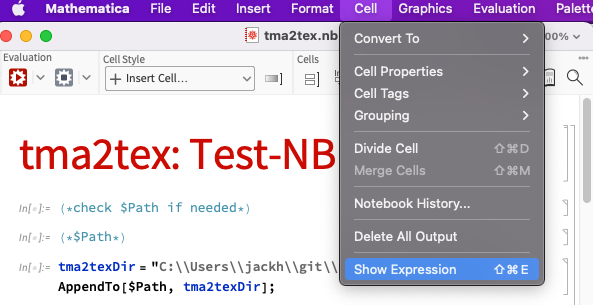
\includegraphics[scale=0.5]{images/introduction/MM-show-expression.png}
    \caption{In Mathematica Desktop, Cell menu and then "Show Expression" reveals ...}
    \label{fig:MM-show-expression}
\end{figure}

\begin{figure}[h]
    \centering
    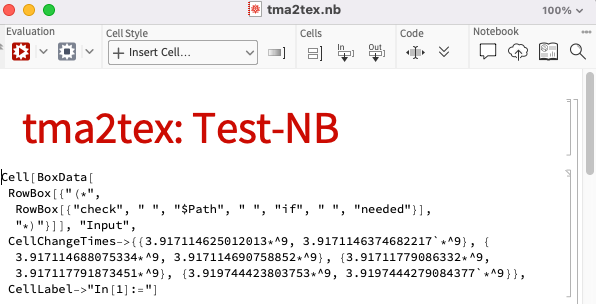
\includegraphics[scale=0.5]{images/introduction/MM-show-expression-1.png}
    \caption{... the lower level expression encoding the typesetting information for what is rendered by the front-end part of the system.}
    \label{fig:MM-show-expression-1}
\end{figure}

As in the FirstTour test notebook, the cells that make up the \lstinline+Notebook[]+ expression (collected in a list), mostly contain in \lstinline+BoxData[]+ and related structures (again, "low-level" representations \cite{noauthor_boxdatawolfram_nodate}), used for typesetting: 'When Wolfram Language expressions are displayed in notebooks, they are represented by two-dimensional typesetting structures of “boxes”' \cite{noauthor_find_nodate} - thus, the typesetting mechanism for Wolfram Language notebooks is the combination of these box structures, also expressions of course, with cell- and notebook-expressions. Any parsing on a notebook therefore takes place in relation to these basic structural elements.

\section{Motivation} \label{document-processing}

The motivation for this project is two-fold: First, \LaTeX is a standard widely used in technical and scientific communities, including journals of relevance to RISC, for example. Second, the native export functionality provided in Mathematica out of the box is not tailored to the Theorema background evaluation of formula representations despite their relevance to Theorema-publications. 

The status quo this project seeks to address is the labor-intensive, manual \LaTeX-preparation of formulae from Theorema notebooks for publication purposes.

\subsection{Need: The \LaTeX-Standard for Academic Publishing in Mathematical Disciplines}

The \LaTeX-typesetting software system is maintained by The Latex Project \cite{noauthor_latex_nodate}: In their words, "\LaTeX is the de facto standard for the communication and publication of scientific documents." \cite{noauthor_latex_nodate-1}

The current thesis is not so much about the format as it is about WL as an engineering tool for the Theorema context and transforming WL/Theorema-notebooks to this format, but the short form history and overview feature list of the system shall be included here: It is based on Donald E. Knuth’s TeX typesetting language, where LaTeX was first developed in 1985 by Leslie Lamport (the "La" in LaTeX), and currently by The LaTeX Project. \cite{noauthor_latex_nodate} 

The Latex Project lists the system's current set of features as follows \cite{noauthor_introduction_nodate}.

\begin{itemize}
    \item Typesetting journal articles, technical reports, books, and slide presentations.
    \item Control over large documents containing sectioning, cross-references, tables and figures.
    \item Typesetting of complex mathematical formulas.
    \item Advanced typesetting of mathematics with AMS (American Mathematical Society) LaTeX.
    \item Automatic generation of bibliographies and indexes.
    \item Multi-lingual typesetting.
    \item Inclusion of artwork, and process or spot colour.
    \item Using PostScript or Metafont fonts.
\end{itemize}

\subsection{Comparison to Existing Functionality in Mathematica} \label{intro:existing-functionality}

Mathematica provides native \LaTeX-export functionality, drawing on AMS-LaTeX, already listed in in the features of the system: AMS-LaTeX extensions are included in the standard LaTeX distribution, where the "amsmath part is an extension package for LaTeX that provides various features to facilitate writing math formulas and to improve the typographical quality of their output." \cite{noauthor_american_nodate} This can be shown by following the steps shown in Figures \ref{fig:MM-save-as} and \ref{fig:MM-to-latex} to save a notebook in in the \LaTeX-format in the "Save as ..." menu.

\begin{figure}[h]
    \centering
    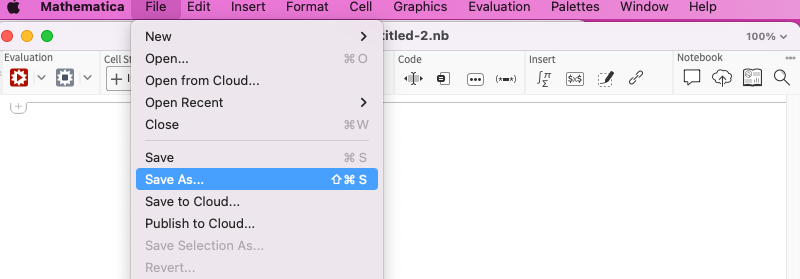
\includegraphics[scale=0.3]{images/introduction/MM-save-as.png}
    \caption{In Mathematica Desktop, file menu and then "Save as ..." leads to the option to save any notebook in \LaTeX format.}
    \label{fig:MM-save-as}
\end{figure}

\begin{figure}[h]
    \centering
    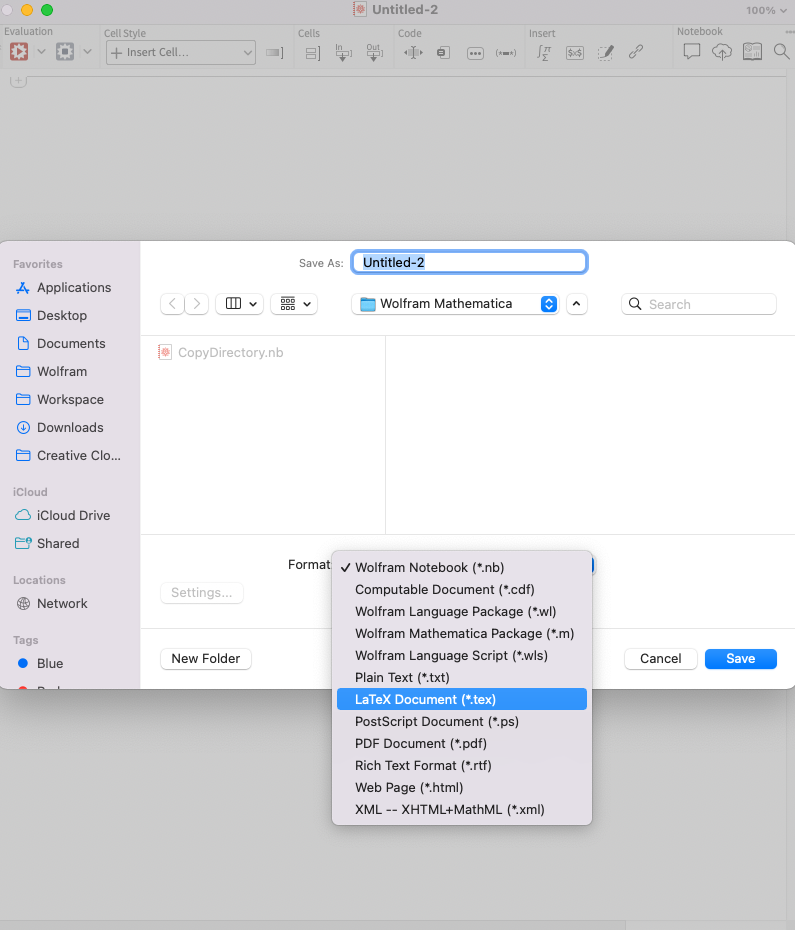
\includegraphics[scale=0.3]{images/introduction/MM-to-latex.png}
    \caption{There are also other export options next to default Mathematica notebook save option, and \LaTeX-Format, the option of interest at this point.}
    \label{fig:MM-to-latex}
\end{figure}

The .TeX-file produced consists of these lines, implementing related package imports and document setup commands.

\begin{verbatim}
%% AMS-LaTeX Created with the Wolfram Language : www.wolfram.com

\documentclass{article}
\usepackage{amsmath, amssymb, graphics, setspace}

\newcommand{\mathsym}[1]{{}}
\newcommand{\unicode}[1]{{}}

\newcounter{mathematicapage}
\begin{document}

\end{document}
\end{LaTeXCode}
\end{program}
\end{verbatim}

Crucially for this project, this native Mathematica solution does not work well for Theorema notebooks, as is easily seen when attempting to use this feature for this project's main test object, FirstTour.nb (provided in the project files), see Figure \ref{}, the PDF-rendering of the native \LaTeX-export (based on FirstTourNativeExport.tex, also provided in the project repository).

The WL (in-notebook) function TeXForm handles the cell-level transformation abd will be the basic Kernel-level functionality that is expanded upon to realize the fundamental transformation functionality in this project, discussed in Section \ref{concept:existing-functionality}.

\section{Development Environment}

\subsection{Tools Used}

In the present work, Mathematica and WolframKernel 14.1 \cite{noauthor_wolfram_nodate} are used throughout: Screenshots of Mathematica for desktop are used to show code evaluation where the frontend is relevant, and IntelliJ IDEA 2022.3.3 \cite{noauthor_intellij_nodate} is used in conjunction with the IntelliJ plugin Wolfram Language by Hal's Corner \cite{noauthor_wolfram_nodate-1} for syntax highlighting, as a guide for setting up a modern WL development environment and note on the present work's tooling: to reproduce this setup, simply install Mathematica (may require a license) and IntelliJ, then the plugin inside of the IntelliJ settings.


\subsection{Platform-(In)dependence}

Core concepts employed in this work to answer the challenge outlined in section \ref{document-processing}, for example pattern matching, related to the symbolic approach already discussed and explored in depth in Sections \ref{pattern-matching-concept} and \ref{pattern-matching-implementation}, are central to WL and the platform as a whole, making backwards and forwards compatibility within the Mathematica ecosystem highly likely. 

Since this work transforms Theorema documents and Theorema extends Wolfram Language, the tool developed here can be applied to vanilla Mathematica notebooks (Wolfram Language under the hood, that is, see section \ref{mm-vs-wl} on the relevant terminology) as well, see section \ref{usage}: The application requires execution on a compatible WL kernel setup. So, while the package is not, in principle, dependent on Theorema, and will simply transform available patterns in the input data - if these are not present, there is limited transformation - it is entirely dependent on the Wolfram Kernel included with Mathematica distributions.

On the level of the operating system, this implementation is platform-\textit{in}dependent and benefits from the Wolfram Language ecosystem setup (see criticisms in Section \ref{tool-chain-with-critique}) the way Theorema does, because (of) "Mathematica programs run without any modifications on essentially all available operating system platforms (Linux, OS X, and Windows), the powerful development group at Wolfram Research that keeps Mathematica being always an up-to-date platform growing into various directions, and the huge group of Mathematica users." \cite[p. 72]{windsteiger_theorema_2013}

\section{Mathematica/Wolfram Language Today}

\subsection{Mathematica vs Wolfram Language (vs Wolfram|Alpha)} \label{mm-vs-wl}

This disambiguation should be helpful for anyone new to the Wolfram ecosystem or "tech stack," as it is currently marketed: \cite{noauthor_wolfram_nodate}

\begin{itemize}
    \item Mathematica: the Desktop application, first introduced in 1988 and available for download in Version 14.1 currently. It is a proprietary technology available at a subscription cost. \cite{noauthor_wolfram_nodate-1}
    \item Wolfram Language: Frequently described as a "symbolic language," it is also the language that the Mathematica kernel is developed in and runs on. WL can be executed inside Mathematica. A Mathematica package typically has the file ending ".wl" (previously ".m") and can be called from inside Mathematica (a Mathematica notebook). It is also in principle closed source \cite{noauthor_wolfram_nodate} and available for licensing.
    \item Wolfram|Alpha: publicly available at no cost in the base version \cite{noauthor_wolframalpha_nodate} this product is sometimes conflated with Mathematica or Wolfram Language due to its public profile. "Wolfram|Alpha's long-term goal is to make all systematic knowledge immediately computable and accessible to everyone." \cite{wolfram_research_inc_about_2024}
\end{itemize}

\subsection{The Wolfram Tool Chain Today and Its Criticisms} \label{tool-chain-with-critique}

Mathematica, first appearing in 1988, is available in Version 14.1 at the time of writing and is being actively developed by Wolfram Research, with "new and improved" features (since Version 13.3) spanning topical categories like Mathematical Computation, Machine Learning and Neural Networks, High-Dimensional Visualization and Astronomy in addition to Core Language, Importing and Exporting and similar base categories. \cite{wolfram_research_export_nodate}] Mathematica, the Desktop application, continues to be Wolfram Research's core product, being marketed as the "world's definitive system for modern technical computing" \cite{noauthor_wolfram_nodate-1} and is distinguished from underlying technologies (Wolfram Language, Wolfram Cloud, Wolfram Knowledgebase, to name a few out of a longer list \cite{noauthor_wolfram_nodate-1}) and contrasts with the more unified platform approach of Wolfram|One \cite{noauthor_wolframone_nodate}, the publicly available Wolfram|Alpha \cite{noauthor_wolframalpha_nodate}, a set of mobile apps \cite{noauthor_wolfram_nodate} and further, more dedicated, products and services.

The size of the program and progress in development is typically measured in number of "in-built functions," that is, functions providing specific functionality, many levels of abstraction higher than the data structure and algorithm oriented functions provided by conventional languages and frameworks: see the following section \ref{computational-language} for the exploration of this idea. The current count of in-built functions, 6602 for the latest major release 14.0 \cite{wolfram_research_inc_summary_2024} and, for the newly released (minor) Version 14.1, up 89 to a new total of 6691 \cite{wolfram_research_inc_yet_2024}, with the trajectory since Version 1.0 in 1988 given in Figure \ref{fig:MM-number-of-built-in-functions}.

\begin{figure}[h]
    \centering
    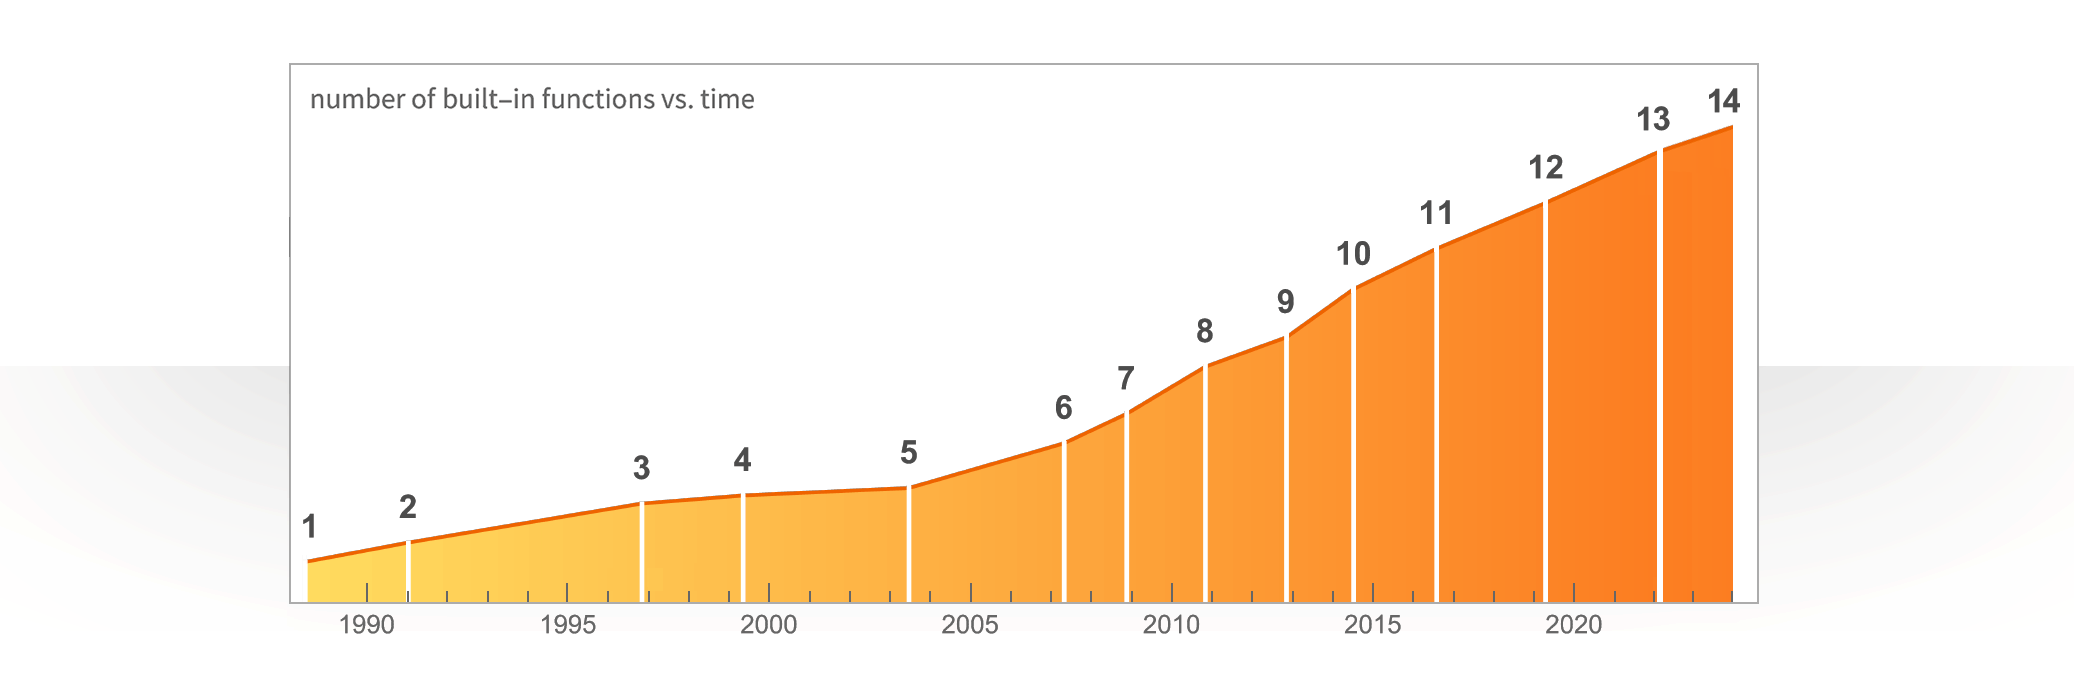
\includegraphics[scale=0.2]{images/introduction/stats-chart.png}
    \caption{In Mathematica Desktop, there are now over 6000 "built-in functions." \cite{noauthor_wolfram_nodate-1}}
    \label{fig:MM-number-of-built-in-functions}
\end{figure}

Criticism of the Wolfram products typically hinge on its closed-source, for-cost nature, though can also be extended to performance and trust in/vendor-lock-in with the company maintaining it, see for example \cite{noauthor_why_2022}. Specifically the former has been addressed as matters of philosophy when it comes to developing a programming language and associated ecosystem: "The simple answer is that large-scale, unified design requires centralized control and sustained effort that we feel is less achievable with free and open-source software" \cite{noauthor_wolfram_nodate} is the official customer facing answer in this proprietary context. A more extensive statement is given in \cite{noauthor_why_2019}, outlining 12 reasons for being closed-source, proprietary and at-cost, similar but slightly different aspects of this question.

Since this chapter started with Bruno Buchberger, I want to bring this particular question to his view, also mentioned in \cite{buchberger_mathematica_1996}: the professional development and marketing of Mathematica "is a feature that may have disadvantages for the research community because the code of the kernel of professional systems is normally not open for the user. On the other hand, it also provides some definite advantages as, for example, professional maintenance, high performance [!], professional software production tools, and - in the case of Mathematica - a fantastic front end." (p. 2) Buchberger was writing to Version 3.0 of Mathematica (in 1996) and is of course speaking of performance as it relates to efficient algorithms implemented in C that the kernel relies on, especially complex calculations "implementing the presently best mathematical methods in various fields" (p. 2), rather than performance as it pertains to the system and Mathematica kernel evaluations as a whole and how these might be compared against fully native C or other, lower level programming languages.

\subsection{How Wolfram Research Views Mathematica/Wolfram Language: The Computational Language Idea} \label{computational-language}

In addressing the question, "What Kind of a Thing Is the Wolfram Language?" \cite{noauthor_what_2019}, Stephen Wolfram, in some position to answer this, as the founder and current CEO of Wolfram Research and originator of the language, espouses the idea of a "computational" language, 'a way to apply the computational paradigm directly to almost anything: we have a language and a notation for doing computational X, for basically any field “X” (from archaeology to zoology, and beyond).' \cite{noauthor_what_2019} Such a multi-purpose tool is differentiated from conventional programming languages in the following way, relevant to the present work.

\begin{displayquote}
First and foremost, it’s that a computational language tries to intrinsically be able to talk about whatever one might think about in a computational way—while a programming language is set up to intrinsically talk only about things one can directly program a computer to do. So for example, a computational language can intrinsically talk about things in the real world—like the planet Mars or New York City or a chocolate chip cookie. A programming language can intrinsically talk only about abstract data structures in a computer. \cite{noauthor_what_2019}
\end{displayquote}

Mars \cite{noauthor_planetwolfram_nodate} and New York City \cite{noauthor_citywolfram_nodate} are examples of entities that can be addressed in WL using the so-called Wolfram Knowledgebase \cite{noauthor_wolfram_nodate}, which also powers Wolfram Alpha \cite{noauthor_curated_nodate}, another Wolfram Research product. The idea of the computational language turns on this easy access to data, as well as pre-built, high-level functions ("while the core of a standard programming language typically has perhaps a few tens of primitive functions built in, the Wolfram Language has more than 5600" at the time of writing \cite{noauthor_what_2019}, in 2019 - now 6602 in Mathematica and WL Version 14.1 \cite{noauthor_story_2024} in 2024, five years on) operating on the WL expression structure. 

This latter and the symbolic notion in an extended sense are seen as key in this presentation; to conclude it, and to give the intuition for the symbolic expressions and how they relate to the central pattern matching approach in Wolfram Language programming for processing expressions, not too different from Regular Expressions matching for strings (of text characters) in more conventional programming contexts: 

\begin{displayquote}
In most standard programming languages, x on its own without a value doesn’t mean anything; it has to stand for some structure in the memory of the computer. But in a computational language, one’s got to be able to have things that are purely symbolic, and that represent, for example, entities in the real world—that one can operate on just like any other kind of data.\cite{noauthor_what_2019}
\end{displayquote}

For the purposes of this work, in document transformation, where it has already been established that the document in question, a Mathematica notebook, is also such a symbolic expression, the idea simply means that any document following the (symbolic, that is expressions-)structure of a Theorema notebook can be processed using the Tma2TeX package: the symbolic in a symbolic expression is to mean something like a class of object, where their particular expression structure ("A foundational idea in the Wolfram Language is that all expressions—whatever they may represent—ultimately have a uniform tree-like structure," \cite{noauthor_expression_nodate}) including the individual expressions (their so-called expression "heads," \cite{noauthor_headwolfram_nodate}) match at the relevant level of abstraction. This level will be the defining mechanism that makes out the pattern matching approach, explored in the Theory chapter (\ref{cha:Theory}) in this work, Section \ref{symbolic-expressions}.

\subsection{The Connection to First Order Predicate Logic} \label{computational-language}

In propositional logic, it is not possible to model predicates like "\( x \) is prime", nor can we reason about statements like "for all \( x \), there exists \( y \) such that \( y \) is a factor of \( x \)". \cite{michael_george_first_2024}

To handle these kinds of statements, predicates and quantifiers need to be introduced; this extended logic is referred to as predicate logic or first-order logic (FOPL):

\[
\phi \in \text{Formulae} ::= \dots \mid P(x_1, x_2, \dots) \mid \forall x, \phi \mid \exists x, \phi
\]

where \( x \) is drawn from a fixed set of variables. \cite{michael_george_first_2024}

Formally, an interpretation can be modeled as a set \( D \) and a function \( I : \text{Pred} \times D \times D \times D \times \dots \to \{T, F\} \) so that one can talk about the truth of a formula in a given interpretation. \cite{michael_george_first_2024}

WL, as a framework, aligns with FOPL, in the sense of the Computational Language concept already explored, leveraging the ability of users to express computational ideas at a high level, in a FOPL style, but providing the means to evaluate  expressions, integrating various data types and a sophisticated set of algorithms and front end, and other aspects of a "system for doing mathematics by computer" \cite{wolfram_research_inc_mathematica_2024}.

As a thesis in the field of Software Engineering, this work will limit its theoretical exploration of the project topic to the technical aspects of the implementation, rather than the mathematical ones, in the following chapter.